\begin{comment}
    ここではグローバーのアルゴリズムについて記述する
\end{comment}

\subsection{グローバーのアルゴリズム}
本節では、データベース探索など、いわゆる探索問題を解く量子アルゴリズムを説明する。
量子探索アルゴリズムは古典の探索アルゴリズムより計算量が少なく、高速であると言われている。
% ここでいう計算量とはオラクルという関数にアクセスする回数で定義されている。

\subsubsection{概要}
このグローバーのアルゴリズムは以下のような流れで行う。
$N$個のデータに対して$O(\sqrt{N})$回の計算量で解を見出すことができる。
古典的な探索アルゴリズムでも同じ計算量を持つ2分探索アルゴリズムがあるが、2分探索アルゴリズムは事前にソートされているデータを扱うため、
ソートされていないデータの探索アルゴリズムではグローバーのアルゴリズムの方が高速である。

このグローバーのアルゴリズムは以下のような流れで行う。
$n$を量子ビット数とすると、$N = 2^n$の要素からなるデータベースから$M$個の解を探索する問題を考え、要素のラベルを$n$桁のビット列$x = x_1 \cdots x_n$とする。

\begin{itemize}
    \item 全ての状態の重ね合わせ状態$\ket{s} = \frac{1}{N} \sum_{x} \ket{x}$を用意する
    \item 演算子$U_w$(解に対する反転操作)を作用させる
    \item 演算子$U_s$($\ket{s}$を対象軸にした反転操作)を作用させる
    \item 2、3を$k$回繰り返す
\end{itemize}

\subsubsection{アルゴリズムの流れ}
まず初めに、全ての状態の重ね合わせ状態$\ket{s} = \frac{1}{\sqrt{N}} \sum_{x} \ket{x}$を用意する。
初期状態$\ket{0}^{\otimes n} = \ket{0 \cdots 0}$に対して全ての量子ビットにアダマール演算子を作用させると、

\begin{equation}
    \begin{split}
      \ket{s} &= H^{\otimes n}\ket{0}^{\otimes n} \\
      &= (H \otimes \cdots \otimes H)\ket{0 \cdots 0} \\
      &= \frac{1}{\sqrt{2^n}}(\ket{0} + \ket{1}) \otimes \cdots \otimes (\ket{0} + \ket{1}) \\
      \ket{s} &= \frac{1}{\sqrt{2^n}} \sum_{x = 0}^{2^n - 1}
    \end{split}
\end{equation}
のように計算できる。

次に解に対する反転操作を作用させる。
入力$\ket{x}$に対して$x$が解なら、$-1$をかけて位相を反転し、解でないならば1をかける。
つまり、単一量子ゲートを以下のように定義する。
\begin{equation}
    \left\{ 
    \begin{alignedat}{2}   
        U_w \ket{x} &= \ket{x} \ (x \ne w) \\
        U_w \ket{w} &= - \ket{w}
    \end{alignedat} 
    \right.
\end{equation}

\begin{equation}
    U_w = I - 2 \sum_{w \in 解} \ket{w}\bra{w}
\end{equation}
$w$は検索したい値である。
これを用いいると、$\ket{s}$は、
\begin{equation}
    \label{eq: Uws}
    \begin{split}
        U_w &= \frac{1}{\sqrt{2^n}} \sum_{x = 0, x \ne w}^{2^n - 1} U_w \ket{x} + \frac{1}{\sqrt{2^n}}U_w \ket{x} \\
        &= \frac{1}{\sqrt{2^n}} \sum_{x = 0, x \ne w}^{2^n - 1} \ket{x} - \frac{1}{\sqrt{2^n}} \ket{w} \\
        U_w \ket{s} &= \ket{s} - \frac{2}{\sqrt{2^n}} \ket{w}
    \end{split}
\end{equation}
のように計算できる。

最後に、$\ket{s}$を対象軸にした反転操作$U_s$を定義する。

\begin{equation}
    \left\{ 
    \begin{alignedat}{2}   
        U_s \ket{x} = 2\bra{s} x \ket{s} - \ket{x} = \frac{2}{\sqrt{2^n}} \ket{x} \\
        U_s \ket{s} = 2 \bra{s} s \ket{s} - \ket{s} = \ket{s}
    \end{alignedat} 
    \right.
\end{equation}

\begin{equation}
    U_s = 2\ket{s}\bra{s} - I
\end{equation}

式(\ref{eq: Uws})より、$U_s$を作用させると、

% \begin{equation}
%     U_s U_w \ket{s} = \ket{s} - \frac{2}{\sqrt{2}}
% \end{equation}

\begin{equation}
    \label{eq: UsUws}
    \begin{split}
        U_s U_w \ket{s} &= \ket{s} - \frac{2}{\sqrt{2}} \left( \frac{2}{\sqrt{2^n}} \ket{s} - \ket{w} \right)\\
        &= \frac{2^n - 4}{2^n} \ket{s} + \frac{2}{\sqrt{2^n}} \ket{w}\\
        &= \frac{2^n - 4}{2^n \sqrt{2^n}} \sum_{x = 0, x \ne w}^{2^n - 1} \ket{x} + \left( \frac{2^n - 4}{2^n \sqrt{2^n}} + \frac{2}{\sqrt{2^n}} \right) \ket{w}\\
        U_s U_w \ket{s} &= \frac{2^n - 4}{2^n \sqrt{2^n}} \sum_{x = 0, x \ne w}^{2^n - 1} \ket{x} + \frac{3 \cdot 2^n - 4}{2^n \sqrt{2^n}} \ket{w}
    \end{split}
\end{equation}

のように計算できる。

$\ket{s}$の時の状態では、$\ket{w}$を測定すると、確率は$\frac{1}{2^n}$となる。
式(\ref{eq: UsUws})から確率が上昇していることがわかる。
この確率を増幅させる操作のことを、反復増幅と呼ぶ。
グローバーのアルゴリズムは、この反復増幅を複数かい行うことにより、$\ket{w}$の確率を1に近づける。


\subsubsection{図を使用しての説明}

$\ket{w}$に直行するベクトル$\ket{w^{\perp}}$を用いた平面を考えると、以下のような状態が得られる。
\begin{equation}
    \ket{w} = \frac{1}{\sqrt{N - M}} \sum^{2^n - 1}_{x = 0, w \neq 0} \ket{x}
\end{equation}

\begin{equation}
    \ket{w^{\perp}} = \frac{1}{\sqrt{M}} \ket{w}
\end{equation}
全ての状態の重ね合せ状態$\ket{s}$は次のように表すことができるので、2次元平面ベクトルであることがわかる。
\begin{equation}
    \label{eq: hgoe}
    \ket{s} = \sqrt{\frac{N - M}{N}} \ket{w^{\perp}} + \sqrt{\frac{M}{N}}\ket{w}
\end{equation}

全ての状態の重ね合わせ状態$\ket{s}$は次のように表せるので、この2次元平面内ベクトルであることがわかる。
% 式(\ref{eq: 3.1})より、$\cos{\frac{\theta}{2}} = \sqrt{\frac{N - M}{N}}, \sin{\frac{\theta}{2}} = \sqrt{\frac{M}{N}}$を満たす角$\theta$を用いれば、
式(\ref{eq: hoge})より、$\cos{\frac{\theta}{2}} = \sqrt{\frac{N - M}{N}}, \sin{\frac{\theta}{2}} = \sqrt{\frac{M}{N}}$を満たす角$\theta$を用いれば、
と表すことができる。
これを図示すると、図\ref{fig:rootate}のようになる。

\begin{equation}
    \ket{s} = \cos{\frac{\theta}{2}} \ket{w^{\perp}} + \sin{\frac{\theta}{2}} \ket{w}
\end{equation}

\begin{figure}[htbp]
    \centering
    \begin{tikzpicture}
        \draw[->,>=stealth,semithick] (-0.5,0)--(4,0)node[above]{$\ket{w^{\perp}}$}; %x軸
        \draw[->,>=stealth,semithick] (0,-0.5)--(0,3.5)node[right]{$\ket{w}$}; %y軸
        \draw (0,0)node[below left]{O}; %原点
        \draw[->] (0,0)--(3, 1.5)node[right]{$\ket{s}$};
        \draw [-](1,0) arc (0:20:1.4);
        \coordinate (thrta_0) at (1,0) node at (thrta_0) [above right] {$\theta / 2$};
    \end{tikzpicture}
    \caption{全ての状態の重ね合わせ状態$\ket{s}$}
    \label{fig:rootate}
\end{figure}

\begin{figure}[htbp]
    \centering
    \begin{tikzpicture}
        \draw[->,>=stealth,semithick] (-0.5,0)--(4,0)node[above]{$\ket{w^{\perp}}$}; %x軸
        \draw[->,>=stealth,semithick] (0,-0.5)--(0,3.5)node[right]{$\ket{w}$}; %y軸
        \draw (0,0)node[below left]{O}; %原点
        \draw[->, dotted] (0,0)--(3, 1.5)node[right]{$\ket{s}$};
        \coordinate (thrta_0) at (1,0) node at (thrta_0) [above right] {$\theta / 2$};
        \draw [-](1,0) arc (0:20:1.4);
        
        \draw[->] (0,0)--(3, -1.5)node[right]{$U_w \ket{s}$};
        \coordinate (thrta_1) at (1,0) node at (thrta_0) [below right] {$\theta / 2$};
        \draw [-](1,0) arc (0:-20:1.4);
    \end{tikzpicture}
    \caption{$\ket{s}$に$U_w$を作用}
    \label{fig:rootate2}
\end{figure}
次に、$\ket{s}$に$U_w$をかけることにより、$\ket{w^{\perp}}$を軸に反転すると、図\ref{fig:rootate2}のようになる。

最後に、$U_s$を作用させることにより、$\ket{s}$を軸に$U_w \ket{s}$を反転させると、図3のようになる。

\begin{figure}[htbp]
    \centering
    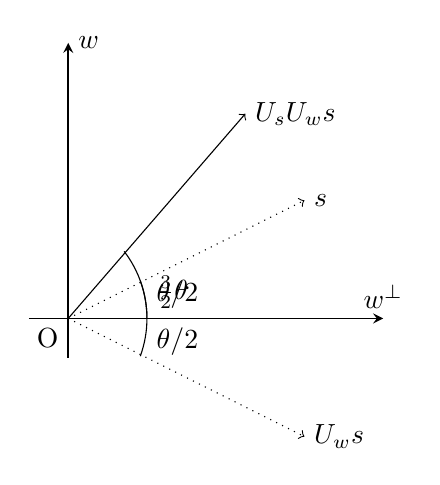
\begin{tikzpicture}
        \draw[->,>=stealth,semithick] (-0.5,0)--(4,0)node[above]{$\ket{w^{\perp}}$}; %x軸
        \draw[->,>=stealth,semithick] (0,-0.5)--(0,3.5)node[right]{$\ket{w}$}; %y軸
        \draw (0,0)node[below left]{O}; %原点
        \draw[->, dotted] (0,0)--(3, 1.5)node[right]{$\ket{s}$};
        \coordinate (thrta_0) at (1,0) node at (thrta_0) [above right] {$\theta / 2$};
        \draw [-](1,0) arc (0:20:1.4);
        
        \draw[->, dotted] (0,0)--(3, -1.5)node[right]{$U_w \ket{s}$};
        \coordinate (thrta_1) at (1,0) node at (thrta_0) [below right] {$\theta / 2$};
        \draw [-](1,0) arc (0:-20:1.4);
        
        \draw[->] (0,0)--(2.25, 2.6)node[right]{$U_s U_w \ket{s}$};
        \coordinate (thrta_0) at (1,0) node at (thrta_1) [above right] {$\frac{3}{2}\theta$};
        \draw [-](1,0) arc (0:37.5:1.4);
    \end{tikzpicture}
    \caption{$U_w\ket{s}$に$U_s$を作用}
    \label{fig:rootate}
\end{figure}

% 以上より、平面ベクトル内で、角度$\theta$だけの回転が行われ、$\ket{w}$を測定する確率が上昇することがわかる。


% \section{最適な$k$の見積もり}
% 最後に、$U_sU_w$を作用させる回数$k$について、最適な回数が幾つなのか調べる。
% 式(3.2)より、グローバーのアルゴリズムを1回施すと、
% \begin{equation}
%     U_sU_w\ket{s} = \cos{\frac{3}{2}\theta}\ket{w^{\perp}} + \sin{\frac{3}{2}\theta}\ket{w}
% \end{equation}
% となる。これを$k$回施すと、
% \begin{equation}
%     (U_sU_w)^k\ket{s} = \cos{\frac{2k+1}{2}\theta} \ket{w^{\perp}} + \sin{\frac{2k+1}{2}\theta} \ket{w}
% \end{equation}
% となる。これを用いて、最終的に$\ket{w}$の確率振幅を1にしたいので、
% % \begin{eqnarray}
% %     \sin{\frac{2k + 1}{2}\theta} = 1 \nonumber \\
% %     \Leftrightarrow	\frac{2k + 1}{2}\theta = \frac{\pi}{2} \nonumber \\
% %     k = \frac{\pi}{2 \theta} 
% % \end{eqnarray}
% \begin{equation}
%     \begin{split}
%             \sin{\frac{2k + 1}{2}\theta} = 1 \\
%             \Leftrightarrow	\frac{2k + 1}{2}\theta = \frac{\pi}{2} \\
%             \therefore k = \frac{\pi}{2 \theta} 
%     \end{split}
% \end{equation}
% となる。よって、$\frac{2k + 1}{2}\theta$が$\frac{\pi}{2}$にもっとも近くなるときは、
% \begin{equation}
%     R = ClosestInteger(\frac{\pi}{2\theta} - \frac{1}{2})
% \end{equation}
% の時である。ここで、$ClosestInteger(...)$は$...$に最も近い整数を表す。

% 最後に、Rの上限を評価する。$\theta > 0$について成り立つ式、
% \begin{equation}
%     \frac{\theta}{2} \geq \sin{\frac{\theta}{2}} = \sqrt{\frac{M}{N}}
% \end{equation}
% を使うと、以下のように表すことができる。
% \begin{equation}
%     R \leq \left( \frac{\pi}{2\theta} - \frac{1}{2} \right) + 1 = \frac{\pi}{2\theta} + \frac{1}{2} \leq \frac{\pi}{4}\sqrt{\frac{N}{M}} + \frac{1}{2}
% \end{equation}
% つまり、Rは$O(\sqrt{N/M})$である。これにより、グローバーのアルゴリズムが$O(\sqrt{N})$で動作することがわかる。
